\chapter{Lavabo - LAVA Board Overseer}
\section{Context}

Since our lab works in a completely autonomous manner thanks to LAVA, we wondered if we could take control of the lab remotely so anyone from Free Electrons could access the boards in the lab from anywhere. lavabo is born from this idea and its goal is to take full remote control of the boards as it is done in LAVA: interface with the serial, control the power supply and serve files to the board. This software also has to be fully compatible with LAVA.

This also find a meaning in Free Electrons sometimes owning only one copy of a board. We still want to automatically test new kernels via LAVA and KernelCI on this board but we might also have to work once in a while on the said board. Before lavabo being developed, engineers had had to physically remove the board from the lab and re-plug all the cables on their desk. This is not an ideal process because, while the board is outside of the lab, the new kernels are not tested on it. At the moment, we have two engineers teleworking far from our Toulouse offices. These engineers might as well work on the board we own only once meaning we have to send them by postal way. Some other engineers also telework from time to time due to business travel and in that case, they would have to take the board (and the needed cables and power supply) with them.

\section{Project}

As presented in the introduction, the goal of lavabo is to take full control of the board. However, LAVA does not yet allow such interaction with boards and thus lavabo needs to interact with boards without interfering with LAVA. If we want to take full control of a board outside of LAVA, we first have to notify LAVA the board is not available for new jobs until further notice. LAVA looks among its dispatchers for online and available devices and if no device is online, drops the jobs it wanted to perform on this device. If there is a device online but is busy, LAVA queues the job. LAVA has an API to interact with  we could use to \textit{put offline} or \textit{online} a board.

Since LAVA already has all means to control the board, we can use the same tools used by LAVA and the configuration file of each board in lavabo to control the board. However, we also need user authentication to deny access to a board when it is already used by an engineer.

\subsection{Implementation}

\begin{figure}[H]
  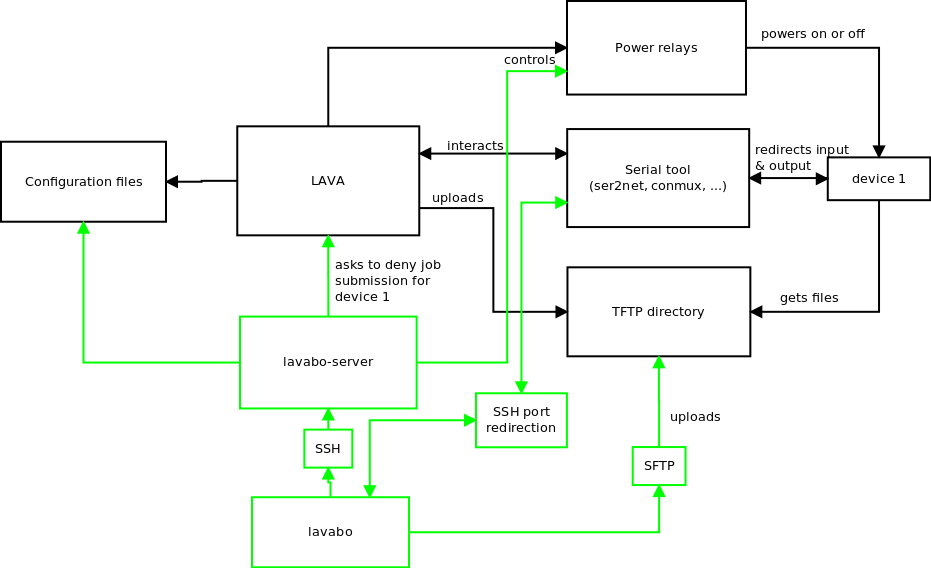
\includegraphics[width=\textwidth]{lavabo-scheme.png}
  \caption{lavabo reuses LAVA tools and configuration files}
\end{figure}

lavabo is a two parts software: a client installed on all engineers' laptop and a server host on the same machine as LAVA. This allows us to use the server part as a bridge to the host to reuse the same tools as LAVA.

All lavabo's logic is in the server part which takes care of calling the right tools directly on the server machine and making the right calls to LAVA's API. It controls the boards and interacts with the LAVA instance to reserve and release a board. The server side of lavabo will be executed every time someone logs in the server machine with a certain user via SSH.

The client is basically connecting via SSH on the server machine with a given user and sending the orders to the server which translates it into commands to execute or calls to make to LAVA's API. Since the client will be connected via SSH on the server with the right user, the server part of lavabo will be executed and the client will interact with the server by writing on server's stdin and reading on server's stdout. This behavior is borrowed from Attic\footnote{\url{https://attic-backup.org/}}. The communication is done via JSON dictionaries so it is easy to parse.

This is perfect for all interactions except the ones that need a continuous stream of data like the serial connection. Writing a terminal functioning through TCP sockets is extremely difficult, but since we already have ser2net exposing serial connections on telnet ports on the server machine, we could do SSH port-forwarding to redirect these telnet ports to ports on engineers' laptop and open a local telnet process connecting to this local port.

\begin{figure}[H]
  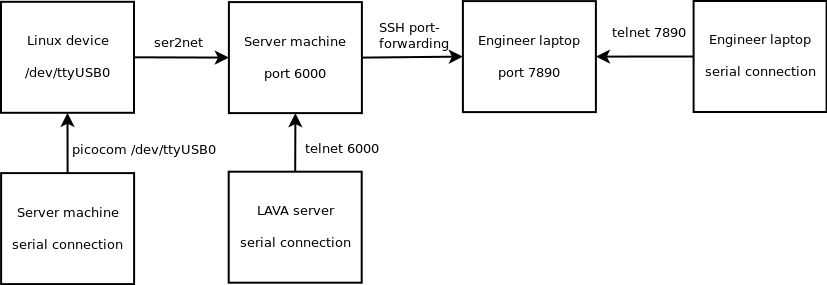
\includegraphics[width=\textwidth]{lavabo-device-port-local_port.png}
  \caption{Different ways to connect to the serial}
\end{figure}

To use a board outside of LAVA, we have to interact with LAVA to tell him it cannot be used anymore. I therefore had to work with LAVA developers to add endpoints for \textit{putting online} (release)\footnote{\url{https://github.com/Linaro/lava-server/commit/2091ac9c3f9305f5a4e083d156c04d1f098ac2fa}} and for \textit{putting offline} (reserve)\footnote{\url{https://github.com/Linaro/lava-server/commit/6da3b4abf0c8a66f746f5a9264fc6ae4ad01f9fc}} boards and an endpoint to get the current status of a board (busy, idle or offline)\footnote{\url{https://github.com/Linaro/lava-server/commit/0d7742db6462fa5c8117556c46b1ce7ec41eda7e}} in LAVA's API.

Now that we know how the client and the server interact and also how the server communicates with LAVA, we need a way to know which boards are in the lab, on which port the serial connection of a board is exposed and what are the commands to control the board's power. Fortunately, all this configuration has already been done in LAVA. To get the list of the available devices, one only needs to list all the files in LAVA devices' configuration file directory. In these configuration file, we can also find all we need to know: what is the port on which the serial connection is exposed, which command to execute to power off and on a board's power. Therefore, lavabo's server part lists and reads LAVA configuration files to avoid duplication of code or configuration.

The last requirement is to serve files to the board. Again, LAVA already has a directory accessible through TFTP from the boards which is one of the mechanisms used to serve files to boards. Therefore, the easiest and most obvious way is to send files from the client to the server and move the files to this directory. We could use either scp or SFTP for this mission. We went with the latter for reasons we expose in the next paragraph.

As explained earlier, we want the server part of lavabo to be automatically launched when a user connects via SSH to the server machine and there are only two means for automatic execution of a code when connecting in SSH:
\begin{itemize}
  \item \mintinline[bgcolor=grey]{console}{$ ssh user@lavabo.server.com "my_command"}

This has to be done on client side and specifies to SSH to execute \mintinline[bgcolor=grey]{bash}{my_command} when connected to the remote. This is a serious security hazard because we do not control what kind of command can be executed in the remote (even if it is not run from root).

  \item use \textit{authorized\_keys} configuration file of ssh with a fixed command to execute

This is set on server side but allows only one command to be set and needs SSH keys of the computer from which the user is trying to connect to the server machine. This command will be executed every time a user is connected via SSH.
\end{itemize}

We obviously chose the second option for security reasons but it also brings an interesting feature: authentication. With the SSH keys, we can now identify who is connected to the server machine and customize the executed command depending on the user. This allows to have a multi-user management. However, this restricts the number of possible commands to be run to only one. scp is not possible when a command is set in authorized\_keys but SFTP is possible when the subsystem sftp is enabled in the configuration of OpenSSH. Trying to connect to the server machine via sftp will actually use the following command to connect: \mintinline[bgcolor=grey]{bash}{ssh user@lavabo.server.com internal-sftp}. Fortunately, in the \textit{authorized\_keys} configuration file, it is possible to retrieve everything that is written after \mintinline[bgcolor=grey]{bash}{ssh user@lavabo.server.com} with the \mintinline[bgcolor=grey]{bash}{$SSH_ORIGINAL_COMMAND} variable\footnote{\url{http://unixwars.blogspot.fr/2014/12/getting-sshoriginalcommand.html}}. Still, the SFTP server needs to be started but we can only have one command to run. Therefore, we pass \mintinline[bgcolor=grey]{bash}{$SSH_ORIGINAL_COMMAND} to lavabo's server part as a parameter and spawns the SFTP server in a subprocess of lavabo's server.\\
There is a small subtlety for the SSH port-forwarding needed to connect to the serial of a board: the command is called even when willing to do only port-forwarding. After some investigation, it turned out the command is run only when the SSH connection is spawning a shell. Fortunately, we do not need a shell on the SSH remote to do port-forwarding so we just had to avoid to spawn a shell with the \textit{-N} argument\footnote{\url{http://linux.die.net/man/1/ssh}} when executing the SSH command in the client.

Since the serial cannot be shared among several sessions, it is essential to guarantee a board can only be used by one engineer at a time. We already have the authentication by SSH key but we need a way to keep track of the user currently using the board to deny access to any new request from other users on this board. To perform such mechanism, we use a small SQLite database. When several engineers work with lavabo, they also have a separate TFTP upload directory so it is easy to know which files to serve to the board.

\subsection{Typical workflow}

\begin{enumerate}
  \item \mintinline[bgcolor=grey]{console}{$ lavabo list}, to get the list of boards in the lab,
  \item \mintinline[bgcolor=grey]{console}{$ lavabo reserve am335x-boneblack_01}, to put the board named \textit{am335x-boneblack\_01} virtually outside of the lab (offline in LAVA),
  \item \mintinline[bgcolor=grey]{console}{$ lavabo upload kernel}, to upload the file name \textit{kernel} in the user's TFTP directory,
  \item \mintinline[bgcolor=grey]{console}{$ lavabo serial am335x-boneblack_01}, to connect to the board named \textit{am335x-boneblack\_01},
  \item \mintinline[bgcolor=grey]{console}{$ lavabo reset am335x-boneblack_01}, to reset power of the board named \textit{am335x-boneblack\_01},
  \item \mintinline[bgcolor=grey]{console}{$ lavabo power-off am335x-boneblack_01}, to power off the board named \textit{am335x-boneblack\_01},
  \item \mintinline[bgcolor=grey]{console}{$ lavabo release am335x-boneblack_01}, to virtually put back the board named \textit{am335x-boneblack\_01} in the lab (online in LAVA);
\end{enumerate}

It is possible to use auto-completion to get the name of a board or to store the name of the board in an environment variable name \mintinline[bgcolor=grey]{bash}{LAVABO_BOARD} with the following line: \mintinline[bgcolor=grey]{console}{$ export LAVABO_BOARD=am335x-boneblack_01}

\section{Conclusion}
This tool is available on the company's GitHub\footnote{\url{https://github.com/free-electrons/lavabo}} under the GNU GPLv2 license and has already been used a fair number of times by the Free Electrons' engineers.

However, there are some possible improvements\footnote{\url{https://github.com/free-electrons/lavabo/issues}}. In the lab, there are some boards which can boot only when using a root filesystem mounted over NFS. However, there is no possibility yet to add an NFS directory to the server machine from lavabo. This problem prevents the use of these boards via lavabo. When following the typical workflow, engineers often forgot to stop \mintinline[bgcolor=grey]{console}{$ lavabo serial am335x-boneblack_01} which means they keep the serial connection open and nobody can use it even if the board is marked as available.
